\section{Cálculos teóricos}

Para empezar a operar el sistema LTI estocástico, es necesario hacer algunos cálculos iniciales, como correlaciones varias.

Como $h(n)$ es la respuesta impulsiva a un filtro FIR de largo $L$, la misma será una secuencia lineal del siguiente tipo:
$h(n) = \{h_0, h_1, \cdots, h_{L-1}\}$. Análogamente, el ecualizador descripto por $w(n)$ también se desarrollará como una secuencia
de largo $M$: $w(n) = \{w_0, w_1, \cdots, w_{M-1}\}$. Por tanto, ambas respuestas son nulas a valores de $n$ negativos (causales) y
superiores a su largo.

Se sabe que $X(n)\in\{-1,1\}$ y, para cada instante distinto, las variables aleatorias son independientes e idénticamente distribuidas,
por lo que tendrán media nula constante. Asumiendo que es un proceso estacionario en sentido amplio, es posible calcular su función de
autocorrelación de la siguiente manera
\begin{align*}
    R_X(k) &= \mathbb{E}[X(n)X(n+k)] =
    \begin{cases}
        \mathbb{E}[\underbrace{X^2(n)}_{ = 1}] & k = 0 \\
        \underbrace{\mathbb{E}[X(n)]\mathbb{E}[X(n+k)]}_{=0} & k \neq 0
    \end{cases}\\
    &= \delta(k).
\end{align*}
Observar que $X(n)$ se trata de un ruido blanco.

Al proceso de salida del filtro FIR se le suma un ruido blanco $V(n)$ de varianza $\sigma^2$ y media nula independiente a $X(n)$,
definiéndose \[Y(n) = (h * X)(n) + V(n) = \sum_{i=1}^{L-1} h(i)X(n - i) + V(n)\] por lo que es posible calcular su función de
autocorrelación de la siguiente manera.

\begin{align*}
    R_Y(k) &= \mathbb{E}[Y(n)Y(n+k)]\\
    &= \mathbb{E}\left[\left(\sum_{i=1}^{L-1} h(i)X(n - i) + V(n)\right)\left(\sum_{j=1}^{L-1} h(j) X(n + k - j) + V(n+k)\right)\right]\\
    &= \sum_{i=1}^{L-1}\sum_{j=1}^{L-1} h(i)h(j) \mathbb{E}[X(n - i)X(n + k - j)] + \mathbb{E}[V(n)V(n + k)]\\
    &= \sum_{i=1}^{L-1}\sum_{j=1}^{L-1} h(i)h(j) R_X(k+i-j) + R_V(k) = \sum_{i=1}^{L-1}\sum_{j=1}^{L-1} h(i)h(j) \delta(k+i-j) + \sigma_V^2\delta(k)\\
    &= \sum_{i=1}^{L-1} h(i)h(k+i) + \sigma_V^2\delta(k) = \sum_{n = 1 - L}^{-1} h(-n)h(k-n) + \sigma_V^2\delta(k) \underset{\substack{\downarrow \\ \tilde{h}(n) = h(-n)}}{=} (\tilde{h}*h)(k) + \sigma_V^2\delta(k)\\
\end{align*}

Se procede a continuación con el cálculo de la correlación cruzada entre $X(n)$ e $Y(n)$.
\begin{align*}
    R_{XY}(k) &= \mathbb{E}[X(n)Y(n+k)] = \mathbb{E}\left[X(n)\left(\sum_{j=1}^{L-1} h(j)X(n + k - j) + V(n+k)\right)\right]\\
    &= \sum_{j=1}^{L-1} h(j) R_X(k-j) = \sum_{j=1}^{L-1} h(j) \delta(k-j) = h(k)
\end{align*}

Los resultados obtenidos son los siguientes:
\begin{align*}
    \boxed{R_X(k) = \delta(k)} &&
    \boxed{R_Y(k) = (\tilde{h} * h)(k) + \sigma_V^2 \delta(k)} &&
    \boxed{R_{XY}(k) = h(k)}
\end{align*}

\section{Elección óptima del filtro ecualizador}
\label{sec:eleccion-optima}

La solución óptima MMSE para los coeficientes del ecualizador debe cumplir con la siguiente expresión:
\begin{equation*}
	\mathbf{R}_Y \mathbf{w}_o = \mathbf{R}_{YX},
\end{equation*}
donde $\mathbf{R}_Y$ es la matriz de Toeplitz de la autocorrelación de $Y$. Luego, la matriz $\mathbf{R}_{YX}$ es:
\[
\mathbf{R}_{YX} = \mathbb{E}
\begin{bmatrix}
	y(n) x(n) \\
	y(n-1) x(n) \\
	\vdots \\
	y(n - M + 1) x(n)
\end{bmatrix}
=
\begin{bmatrix}
	R_{YX}(0) \\
	R_{YX}(1) \\
	\vdots \\
	R_{YX}(M-1)
\end{bmatrix}
=
\begin{bmatrix}
	h(0) \\
	h(-1) \\
	\vdots \\
	h(-M+1)
\end{bmatrix}
=
\begin{bmatrix}
	h(0) \\
	0 \\
	\vdots \\
	0
\end{bmatrix}
\]

Finalmente $\mathbf{w}_o$ es un vector que se obtiene de operar de la siguiente manera con las matrices previamente mencionadas
\begin{equation*}
	\mathbf{w}_o = \mathbf{R}_Y^{-1} \cdot \mathbf{R}_{YX}.
\end{equation*}

\section{Simulación del sistema}

Como se demuestra en la Sección~\ref{sec:eleccion-optima}, las matrices con las que se calculan los coeficientes óptimos para el ecualizador dependen solamente de los coeficientes del modelo del canal. Luego se simuló la secuencia $X(n)$ y en base a ella se calcularon las secuencias $Y(n)$ y $Z(n)$ usando la función \verb|filter| con $\mathbf{h}$ y $\mathbf{w}_o$. El ruido $V(n)$ que se añade a la distorsión causada por el canal es un ruido blanco gaussiano de media nula y varianza $\sigma_V^2 = 0.005$. Los coeficientes del filtro $h(n)$ que distorsiona la señal son ${1, 0.6, 0.2, -0.2, 0.1, 0.05}$.

La figura~\ref{fig:ej3_x} muestra como la autocorrelación de $X(n)$ resulta en algo similar a una delta en el origen y la PSD resulta ruidosa, pero relativamente constante.

\begin{figure}[!hbp]
	\centering
    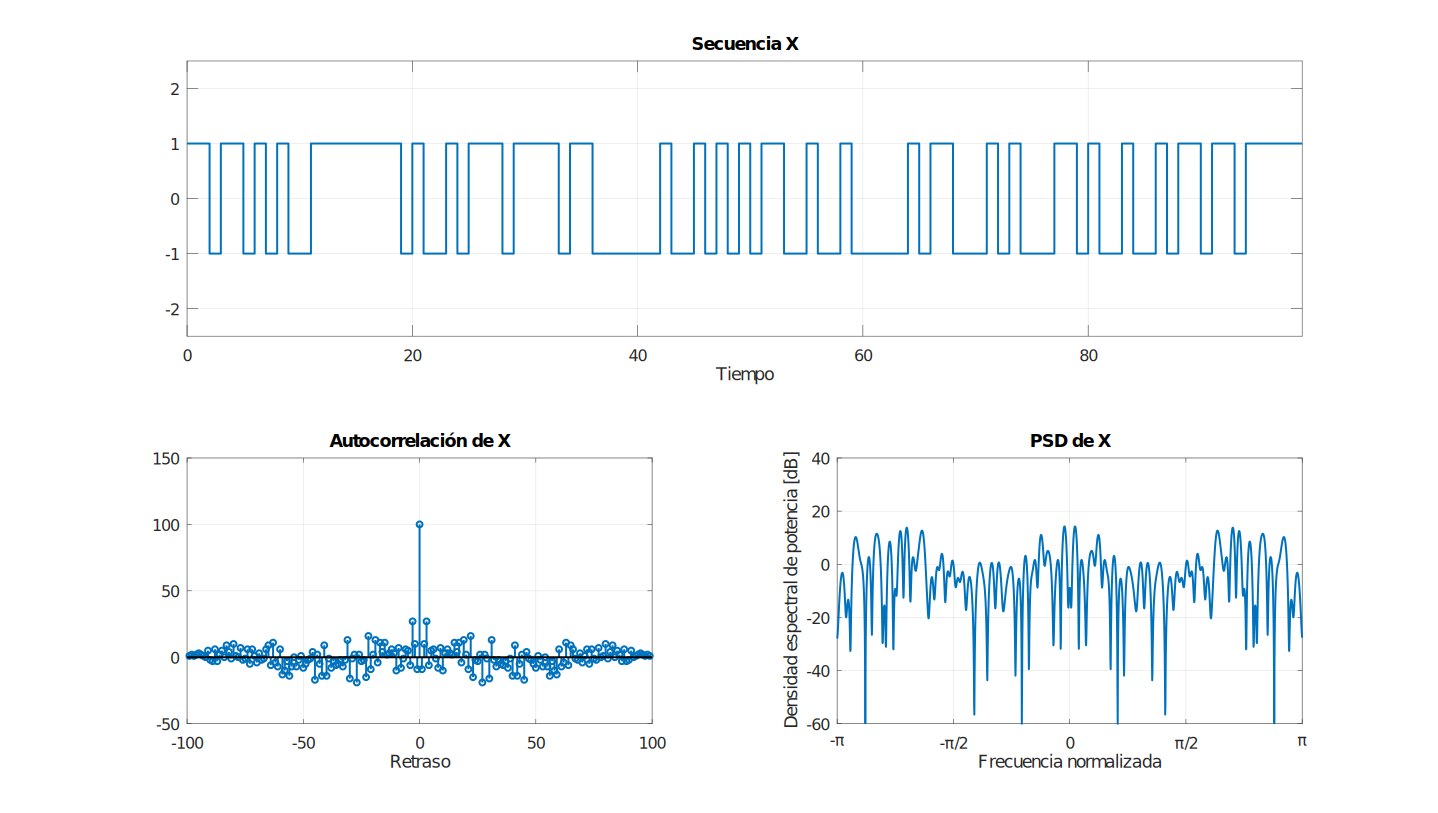
\includegraphics[width=1\linewidth,trim=4cm 0 4cm 0,clip]{img/ej3_x.pdf}
	\caption{Secuencia, autocorrelación y PSD de $X(n)$.}
	\label{fig:ej3_x}
\end{figure}

En la figura~\ref{fig:ej3_y} se observan los atributos de la secuencia $Y(n)$, es decir cómo termina $X(n)$ una vez que atraviesa el canal. Como era de esperar, la señal se distorsiona considerablemente, ya que tanto la secuencia, como su autocorrelación y PSD difieren mucho de $X(n)$.

\begin{figure}[!hbp]
	\centering
	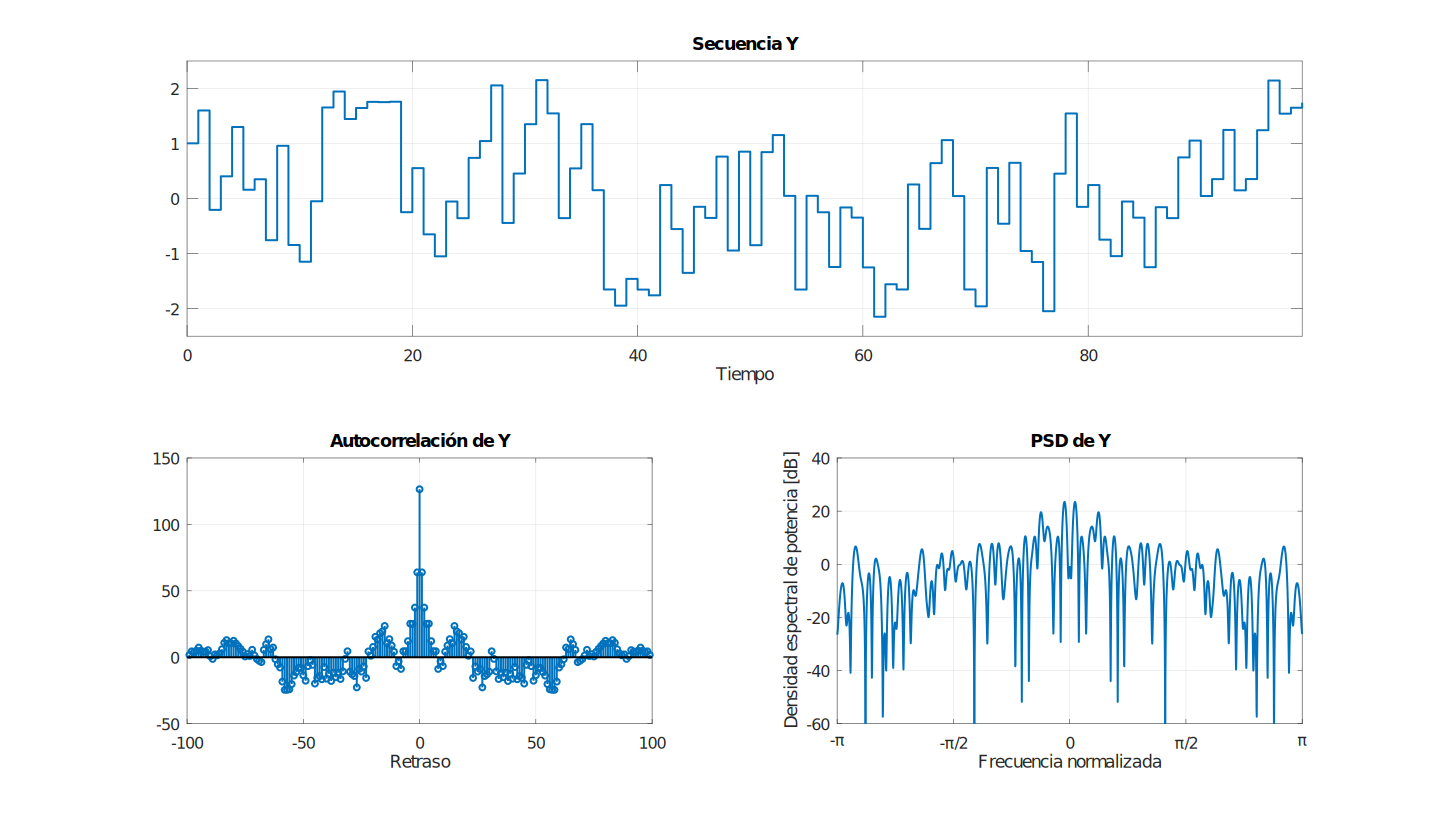
\includegraphics[width=1\linewidth,trim=4cm 0 4cm 0,clip]{img/ej3_y.pdf}
	\caption{Secuencia, autocorrelación y PSD de $Y(n)$.}
	\label{fig:ej3_y}
\end{figure}

Por último, la figura~\ref{fig:ej3_z} muestra una secuencia casi idéntica a la de entrada, demostrando que el ecualizador funcionó correctamente.

\begin{figure}[!hbp]
	\centering
	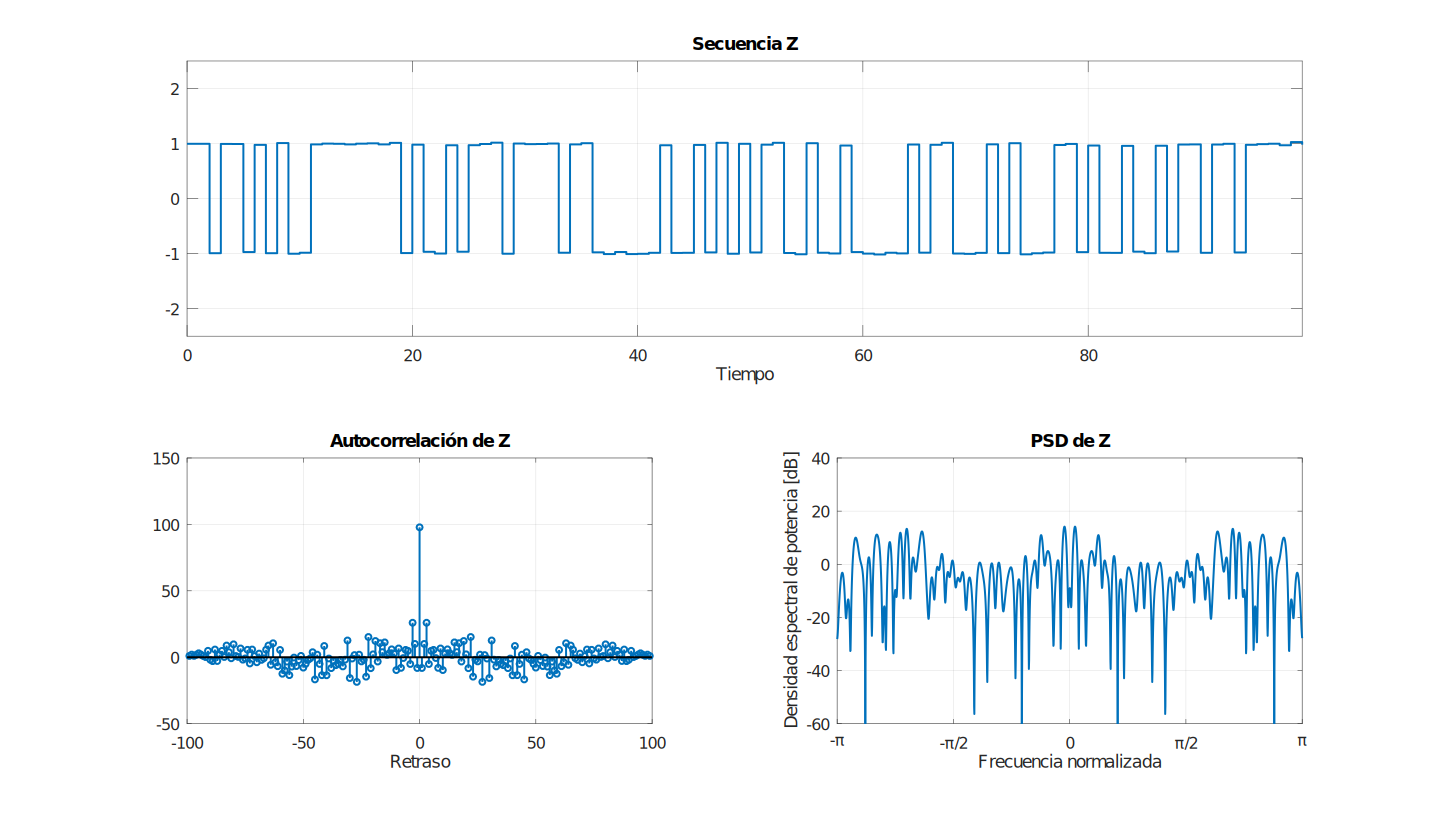
\includegraphics[width=1\linewidth,trim=4cm 0 4cm 0,clip]{img/ej3_z.pdf}
	\caption{Secuencia, autocorrelación y PSD de $Z(n)$.}
	\label{fig:ej3_z}
\end{figure}

En la figura~\ref{fig:ej3_coef} se muestra una comparación de los coeficientes del modelo del canal y los coeficientes del ecualizador obtenidos.

\begin{figure}[!hbp]
	\centering
	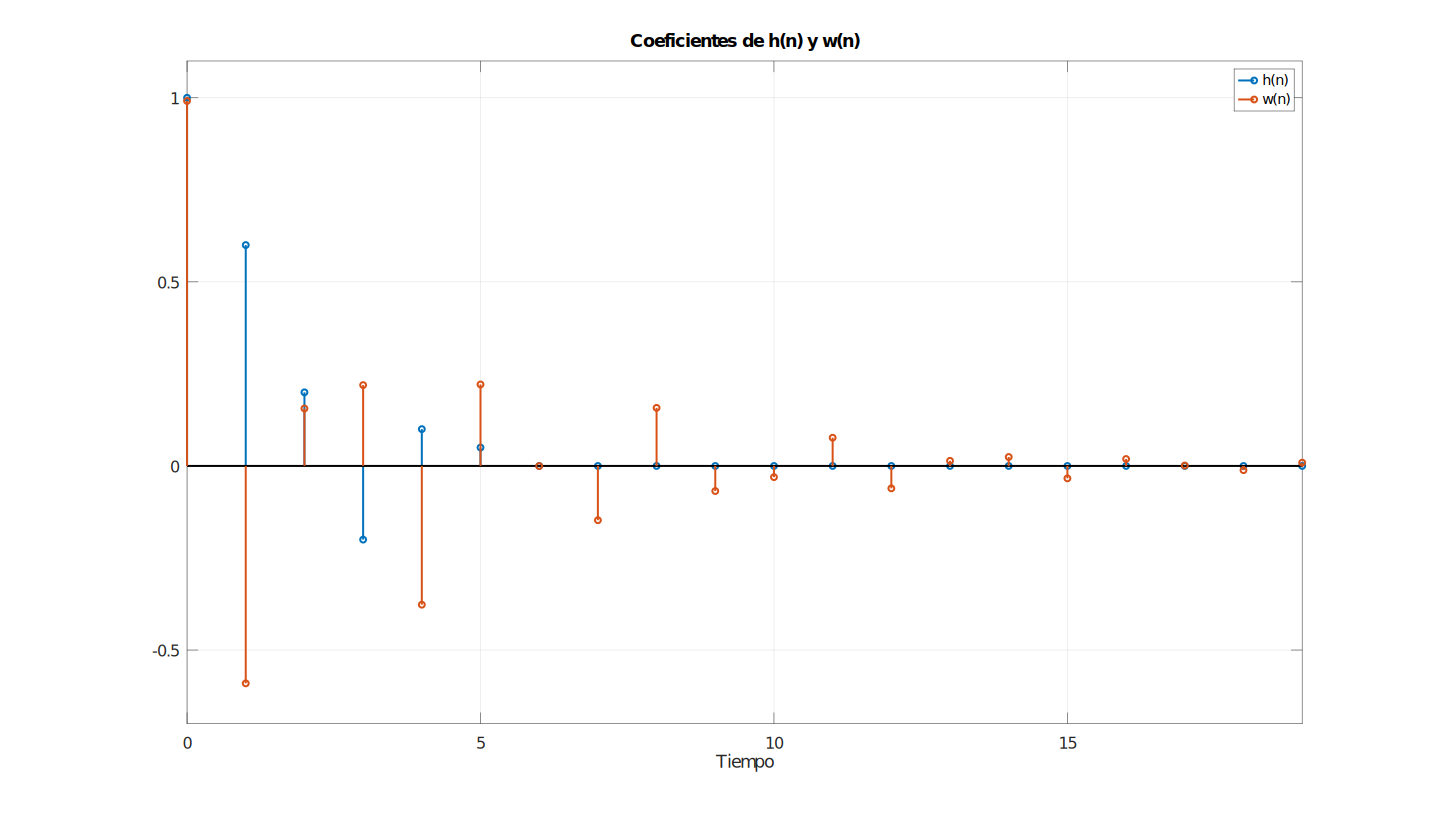
\includegraphics[width=\linewidth,trim=4cm 0 4cm 0,clip]{img/ej3_coef.pdf}
	\caption{Comparación de $h$ y $w$.}
	\label{fig:ej3_coef}
\end{figure}

\clearpage
\section{Variación del largo del filtro ecualizador}

En esta instancia se analiza cómo la longitud del filtro ecualizador afecta la calidad de la señal de salida. Para eso se toman distintos largos del filtro ecualizador (2, 5, 10, 30) y se grafican los coeficientes del filtro ecualizador resultantes, la convolución entre el filtro y el canal $\mathbf{w}_o * \mathbf{h}$ y por último las respuestas en frecuencia $|H(w)|, |W(w)|$ y $|H(w)| \cdot |W(w)|$ (figuras~\ref{fig:ej4_2_coef},~\ref{fig:ej4_5_coef},~\ref{fig:ej4_10_coef} y~\ref{fig:ej4_30_coef}). Además se grafican las secuencias $Z(n)$ resultantes en las figuras~\ref{fig:ej4_2_z},~\ref{fig:ej4_5_z},~\ref{fig:ej4_10_z} y~\ref{fig:ej4_30_z} para cada largo del ecualizador. Esto sirve para observar qué tanto se parece la señal resultante $Z(n)$ a la entrada $X(n)$. Notar que tanto $X(n)$ como la señal distorsionada y ruidosa $Y(n)$ son las mismas que se utilizaron en el análisis previo, siendo las dadas en las figuras~\ref{fig:ej3_x} y~\ref{fig:ej3_y}, respectivamente.

Se nota que a medida que $M$ crece, $Z(n)$ se parece cada vez más a $X(n)$, atenuándose todo efecto inducido por el canal. Para un $M$ chico, por ejemplo $M = 2$ en la figura~\ref{fig:ej4_2_z}, no hay suficiente información en el ecualizador para revertir los cambios que hace el canal. Por otro lado, llega un punto en el que aumentar $M$ no tiene un efecto diferencial sobre la salida, por lo que no tiene sentido seguir aumentándolo ya que significa más gasto computacional. En particular, casi no se observan cambios entre las señales ecualizadas obtenidas para $M = 20$ (figura~\ref{fig:ej3_z}) y $M = 30$ (figura~\ref{fig:ej4_30_z}). Incluso para $M = 10$, si bien la distorsión es más apreciable, la similitud entre $X(n)$ y $Z(n)$ es muy alta.

Esto mismo se puede visualizar en las figuras del sistema en cascada. Recordar que $Z(n) = \mathbf{w}_o * \mathbf{h} * X(n) + \mathbf{w}_o * V(n)$, por lo que es deseable que $\mathbf{w}_o * \mathbf{h} = \delta(k)$---el sistema identidad---, para que $Z(n) \approx X(n)$. Dicho otra manera, que la respuesta en frecuencia del sistema en cascada sea un filtro \emph{pasa-todo}. En la figura~\ref{fig:ej4_30_coef} se aprecian estos atributos mencionados. Mientras que para filtros ecualizadores no lo suficientemente largos, la convolución entre $h(n)$ y $w(n)$ es cercana pero no igual a una delta en el origen, y la respuesta en frecuencia del sistema combinado ($|H(\omega)| \cdot |W(\omega)|$) no tiene magnitud exactamente 1 (\qty{0}{\dB}), como se observa en la figura~\ref{fig:ej4_2_coef}.

En resumen, hay que encontrar una relación de compromiso entre el largo del ecualizador y la calidad de la señal de salida, para obtener algo fiel a la entrada sin tener que hacer cálculos en vano.

\begin{figure}[!hbp]
	\centering
	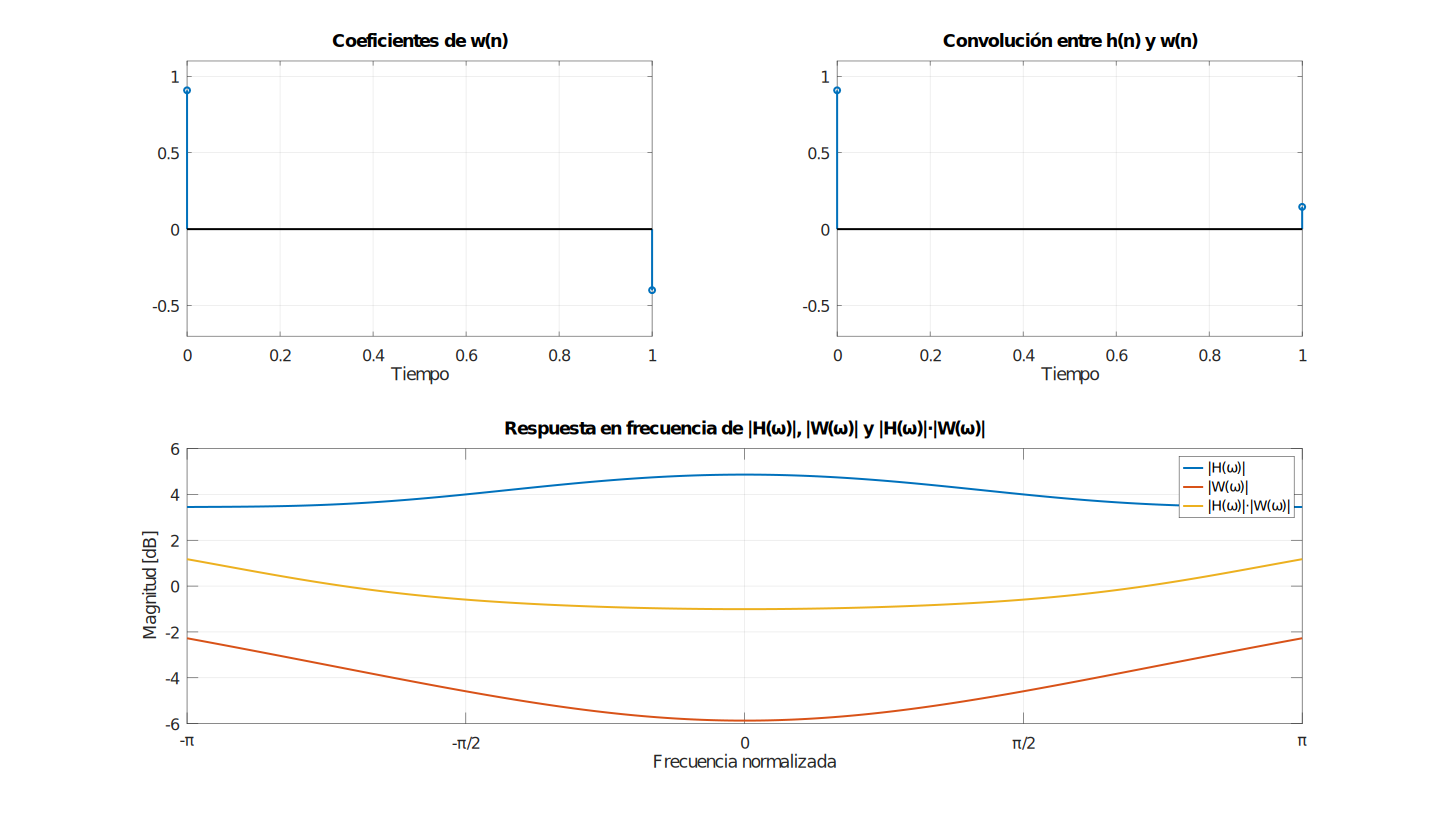
\includegraphics[width=1\linewidth,trim=4cm 0 4cm 0,clip]{img/ej4_2_coef.pdf}
	\caption{Filtro, sistema en cascada y respuestas en frecuencia para M = 2.}
	\label{fig:ej4_2_coef}
\end{figure}

\begin{figure}[!hbp]
	\centering
	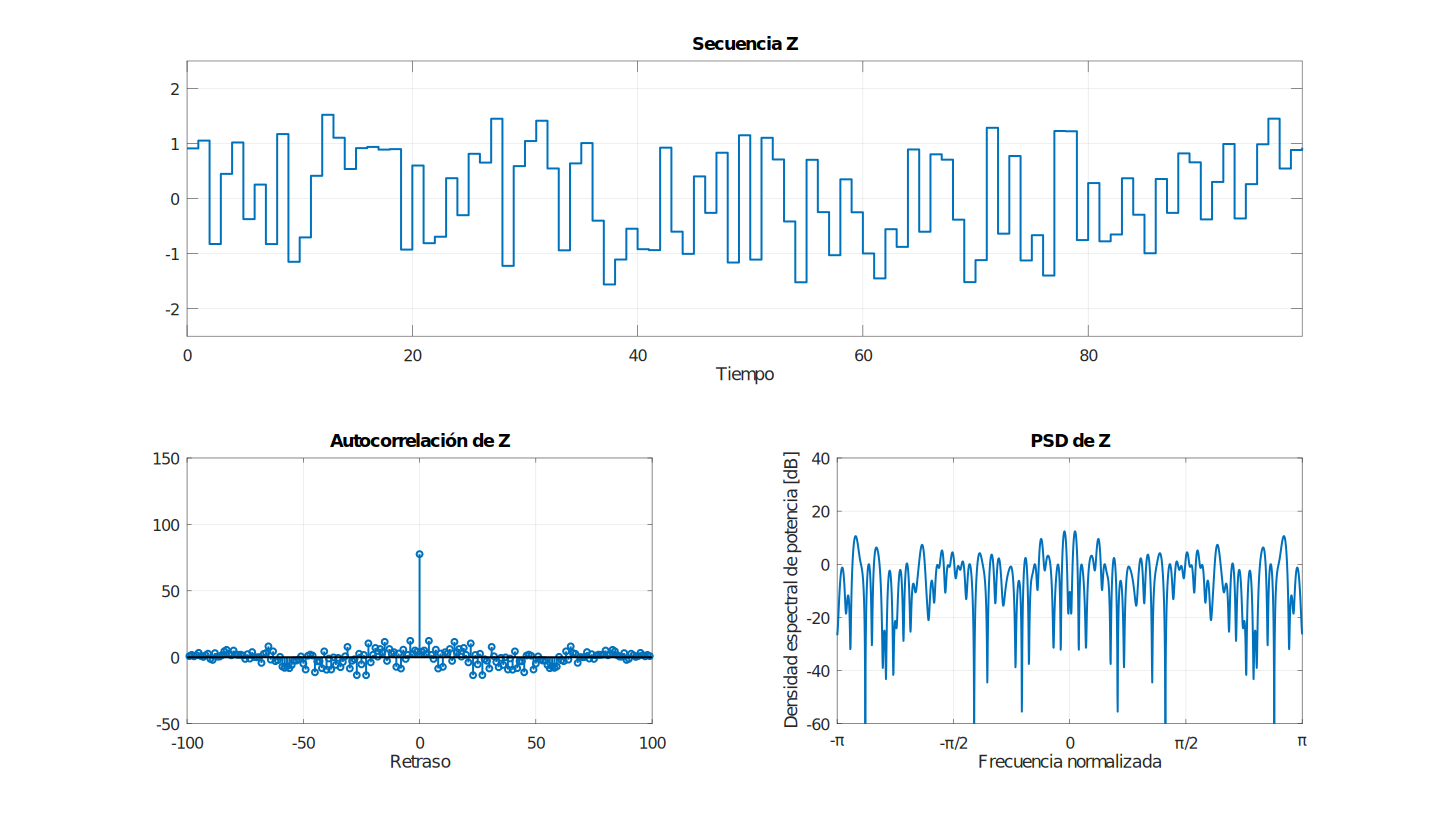
\includegraphics[width=1\linewidth,trim=4cm 0 4cm 0,clip]{img/ej4_2_z.pdf}
	\caption{Secuencia Z(n) resultante para M = 2.}
	\label{fig:ej4_2_z}
\end{figure}

\begin{figure}[!hbp]
	\centering
	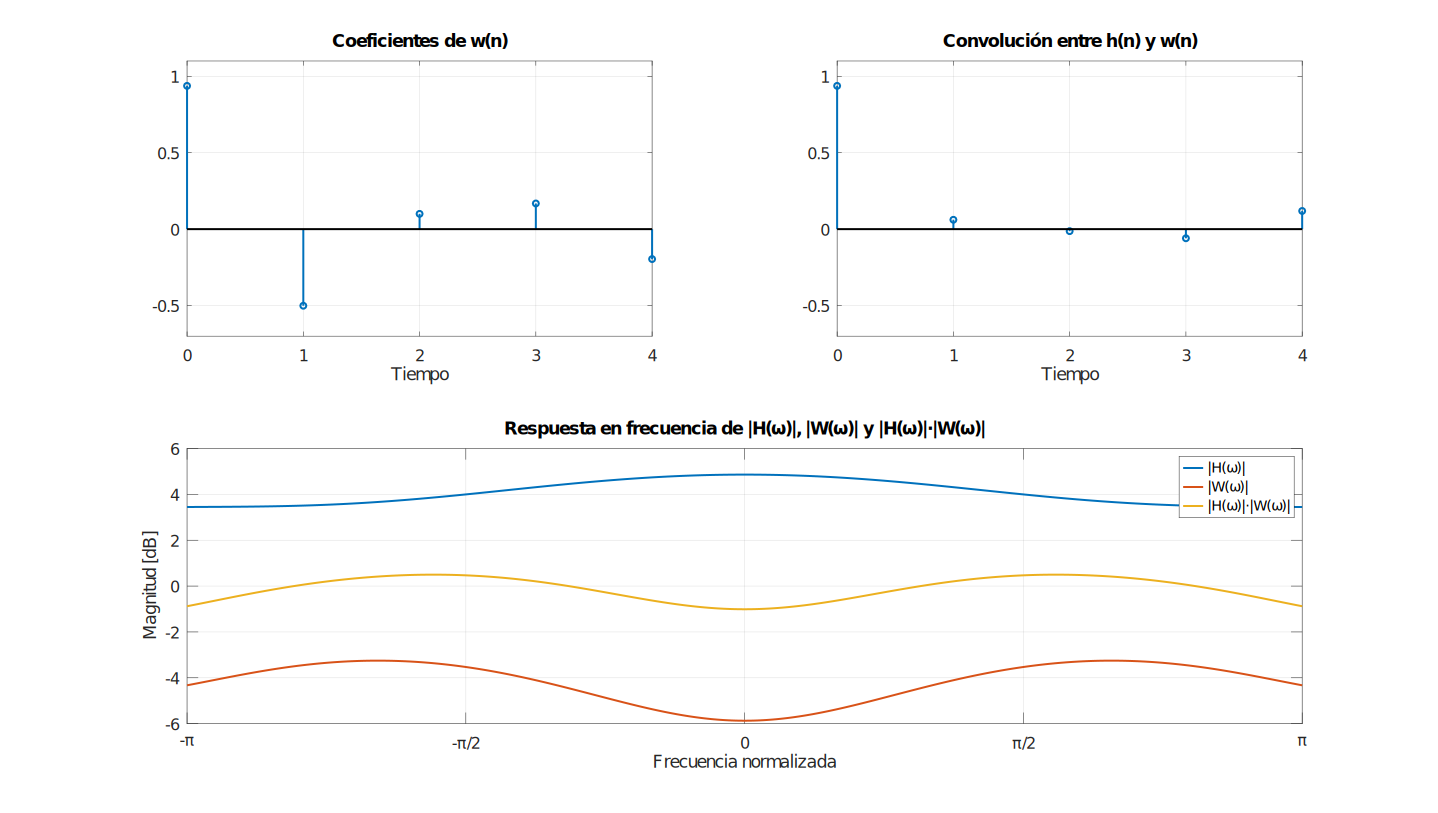
\includegraphics[width=1\linewidth,trim=4cm 0 4cm 0,clip]{img/ej4_5_coef.pdf}
	\caption{Filtro, sistema en cascada y respuestas en frecuencia para M = 5.}
	\label{fig:ej4_5_coef}
\end{figure}

\begin{figure}[!hbp]
	\centering
	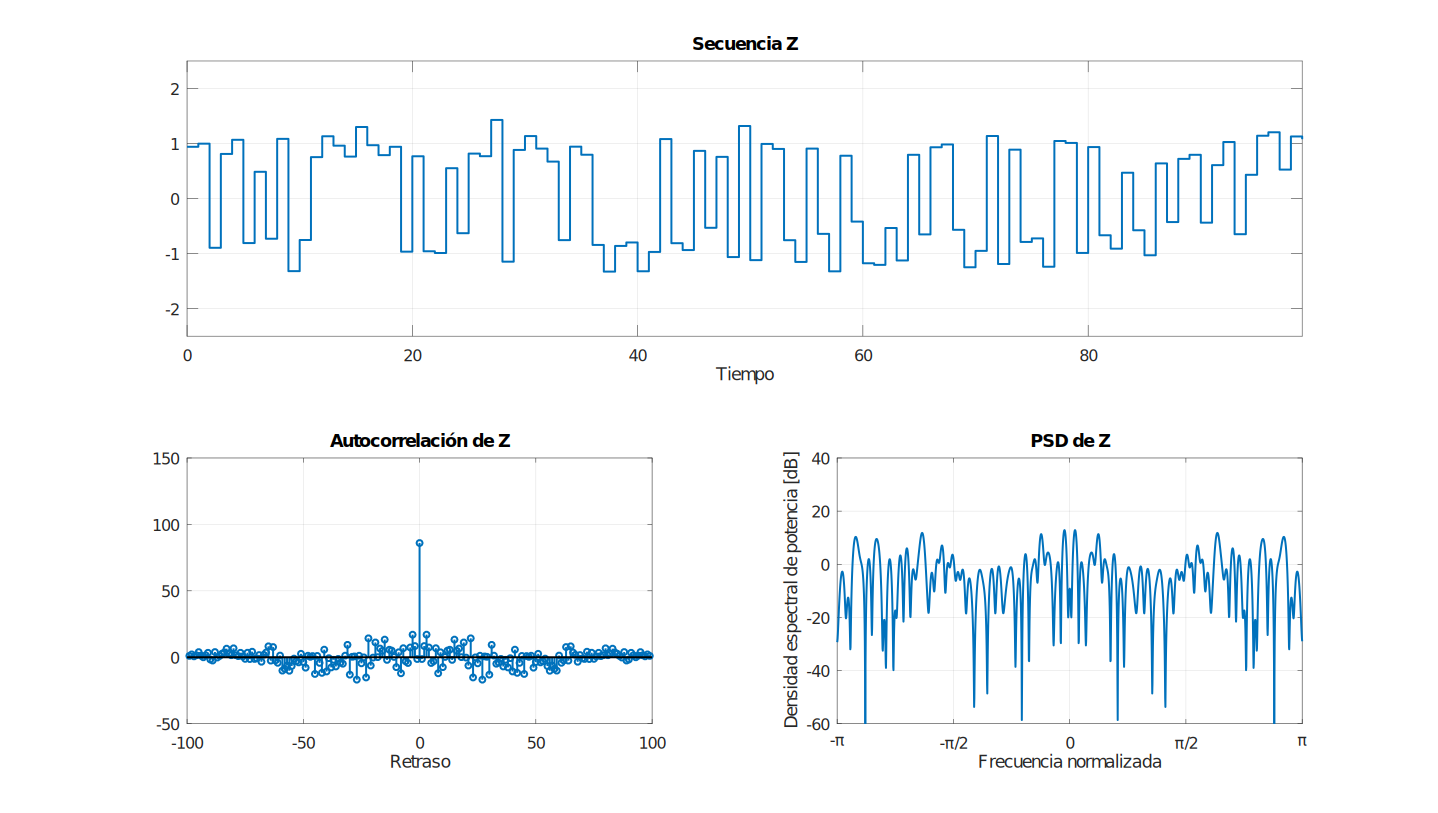
\includegraphics[width=1\linewidth,trim=4cm 0 4cm 0,clip]{img/ej4_5_z.pdf}
	\caption{Secuencia Z(n) resultante para M = 5.}
	\label{fig:ej4_5_z}
\end{figure}

\begin{figure}[!hbp]
	\centering
	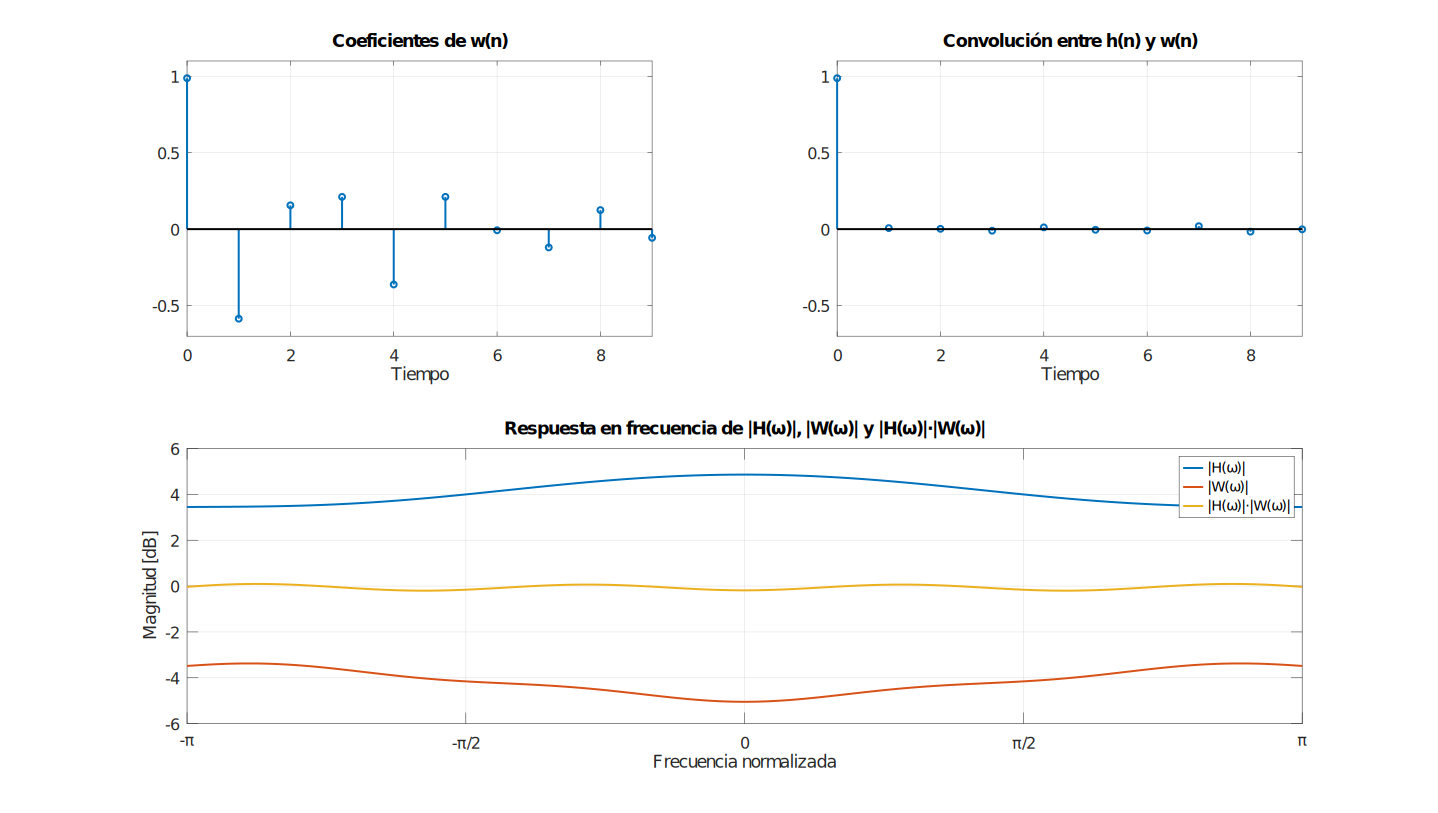
\includegraphics[width=1\linewidth,trim=4cm 0 4cm 0,clip]{img/ej4_10_coef.pdf}
	\caption{Filtro, sistema en cascada y respuestas en frecuencia para M = 10.}
	\label{fig:ej4_10_coef}
\end{figure}

\begin{figure}[!hbp]
	\centering
	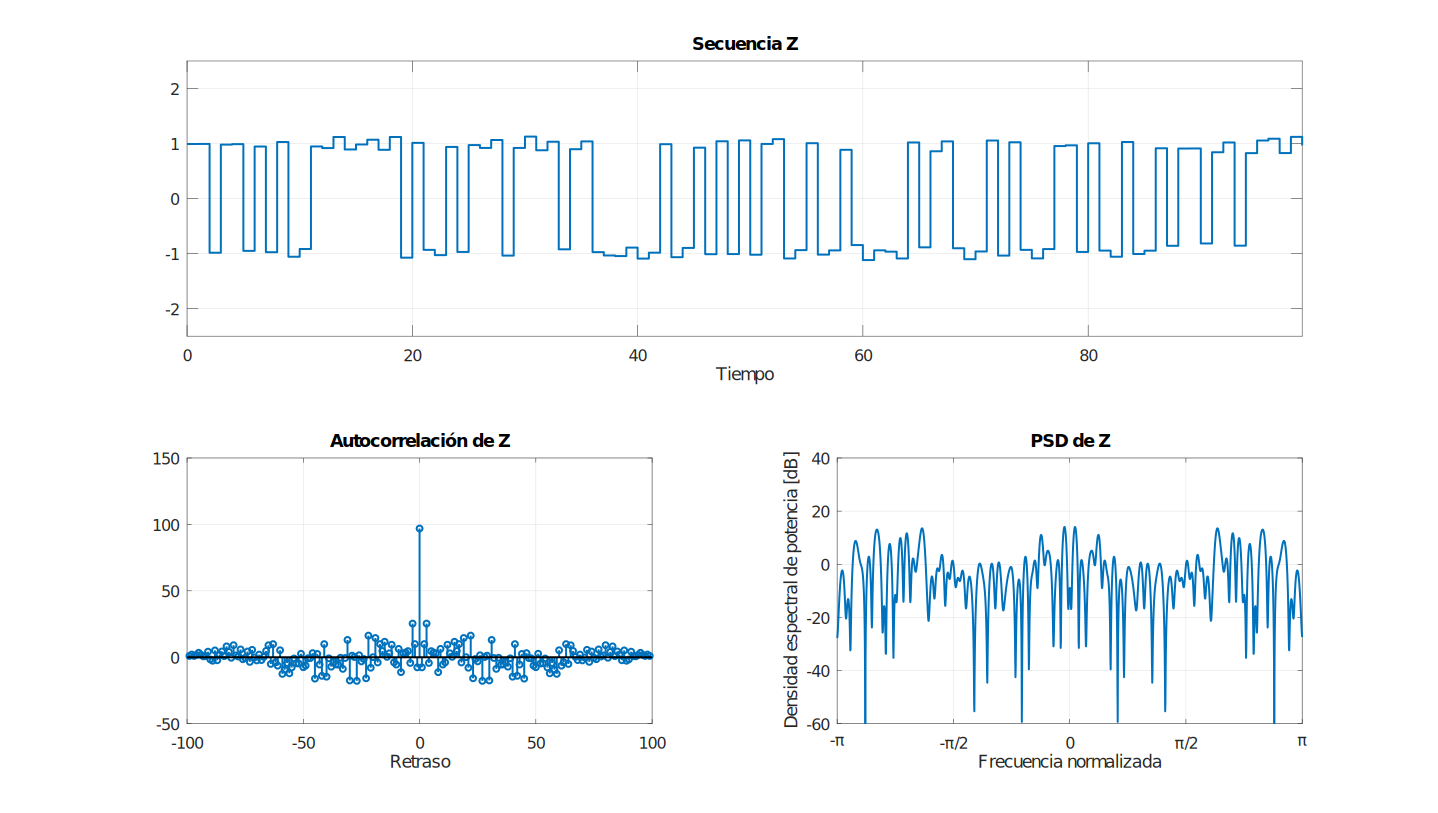
\includegraphics[width=1\linewidth,trim=4cm 0 4cm 0,clip]{img/ej4_10_z.pdf}
	\caption{Secuencia Z(n) resultante para M = 10.}
	\label{fig:ej4_10_z}
\end{figure}

\begin{figure}[!hbp]
	\centering
	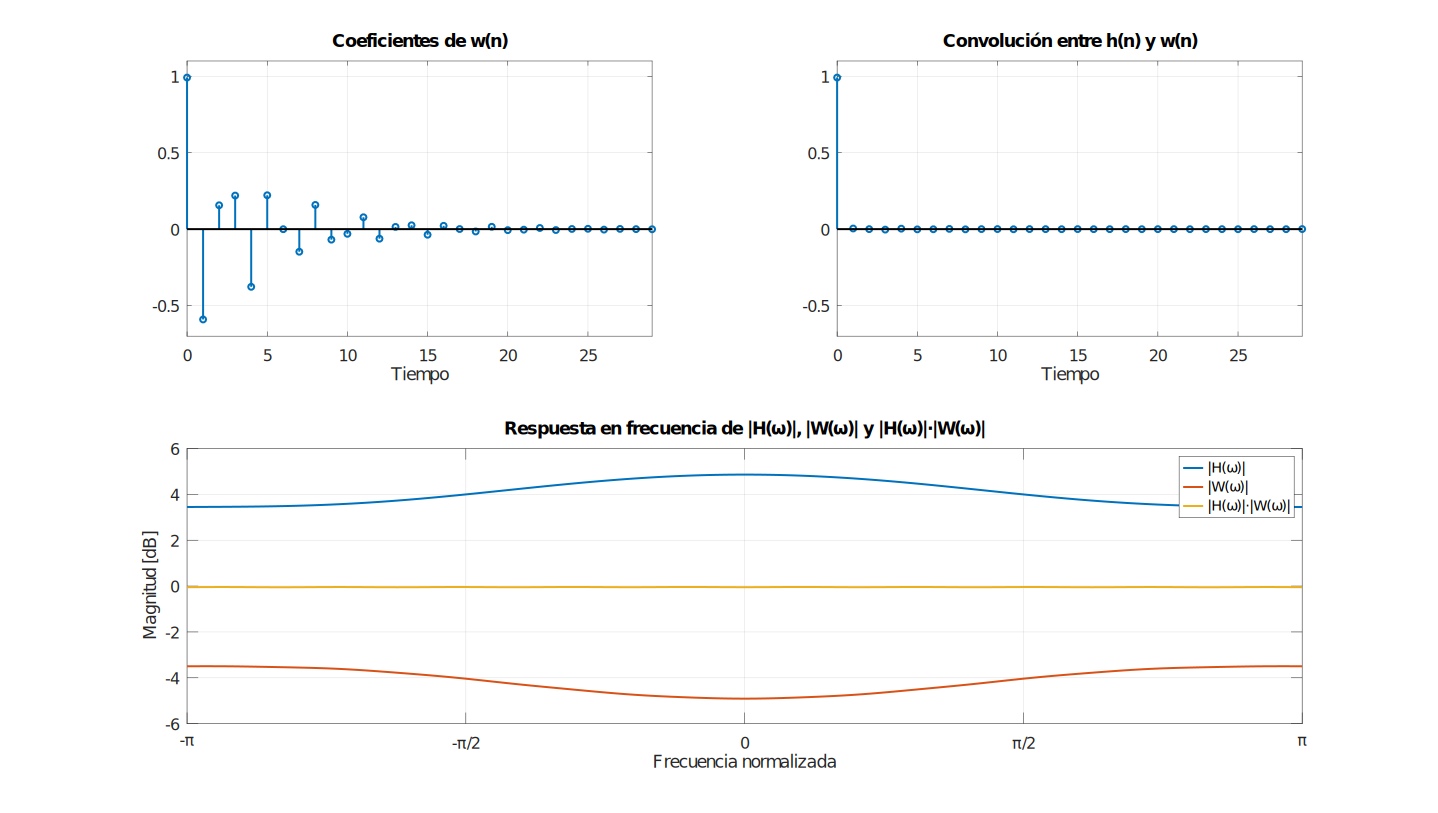
\includegraphics[width=1\linewidth,trim=4cm 0 4cm 0,clip]{img/ej4_30_coef.pdf}
	\caption{Filtro, sistema en cascada y respuestas en frecuencia para M = 30.}
	\label{fig:ej4_30_coef}
\end{figure}

\begin{figure}[!hbp]
	\centering
	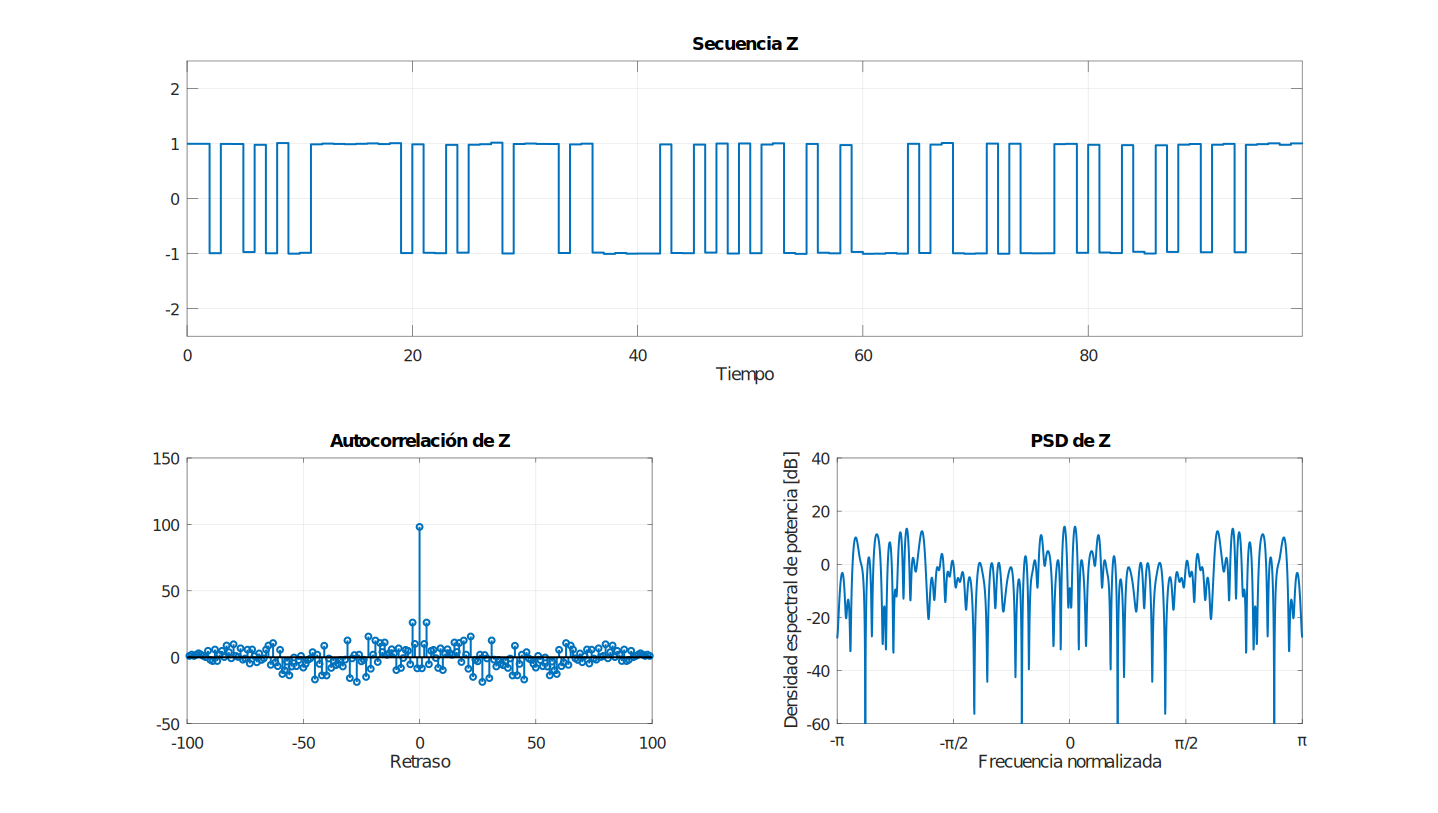
\includegraphics[width=1\linewidth,trim=4cm 0 4cm 0,clip]{img/ej4_30_z.pdf}
	\caption{Secuencia Z(n) resultante para M = 30.}
	\label{fig:ej4_30_z}
\end{figure}

